%!TEX root = ../../main.tex

% Processo de aprendizado OK
% Tarefa de classificação binária
% Divisão dos Dados
% Explicação do método holdout
% Parâmetros e hiperparâmetros
% Métricas Utilizadas - cenários balanceados e desbalanceados

A tarefa de aprendizado abordada neste trabalho consiste em uma tarefa de classificação binária. Neste contexto, uma imagem de $256 \times 256$ \emph{pixels} composta por duas assinaturas manuscritas, na qual a primeira delas representa uma assinatura de referência genuína e a segunda compreende uma assinatura a ser verificada. A saída desejada é a predição da autenticidade da segunda assinatura que, por ser uma tarefa de classificação binária, poderá possuir somente dois valores, \emph{autêntica} ou \emph{forjada}. Esse processo de aprendizado pode ser visualizado na Figura \ref{fig:esquema-solucao}.

\begin{figure}[h!]
  \centering
  \caption{Uma visão geral do processo de aprendizado.}
  \label{fig:esquema-solucao}
  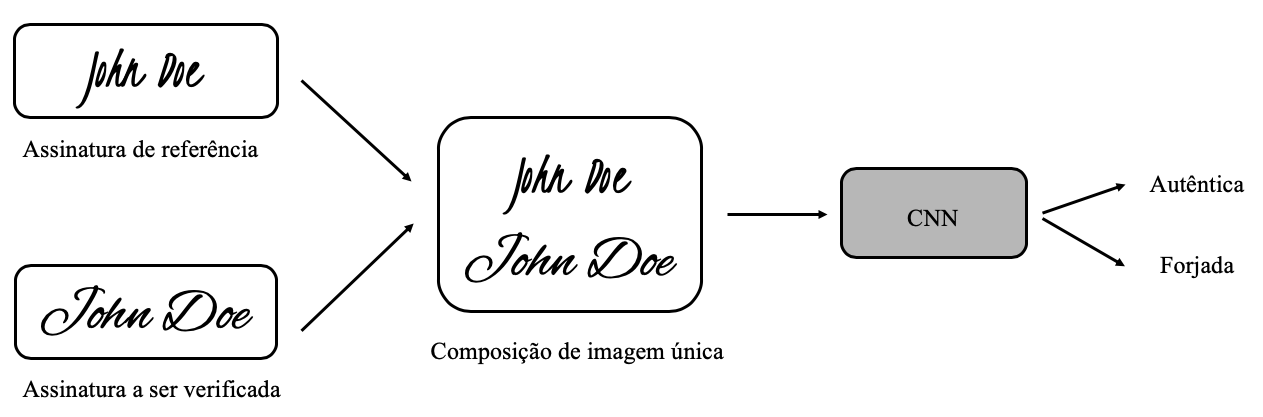
\includegraphics[width=\textwidth]{imgs/esquema-solucao}
\end{figure}

O treinamento e teste das CNNs seguirão o método \emph{holdout} de validação cruzada, em que $70\%$ dos dados serão utilizados no treino e ajuste de parâmetros, enquanto $20\%$ dos dados serão aproveitados para o processo de teste das redes, com vista a capturar o poder de generalização dos modelos considerados. Os $10\%$ de dados restantes, serão utilizados para a validação dos modelos durante o processo de treinamento \cite{brink}.

Os modelos propostos serão avaliados perante as métricas de desempenho de \emph{Acurácia} e \emph{F-score}. A acurácia indica a proporção de predições corretas inferidas pelos modelos. O \emph{F-score}, por sua vez, é calculado pela média harmônica da precisão e da revocação, que assumirá valores diferentes dependendo do balanceamento do conjunto de dados apresentando ao modelo.

Para um \emph{dataset} balanceado, os cálculos da precisão e revocação serão realizados através da técnica de \emph{macro-average}, enquanto para um \emph{dataset} desbalanceado, esses valores serão determinados através do \emph{micro-average}. Nas equações \ref{eq:precision} e \ref{eq:recall} estão demonstrados os valores de precisão ($P$) e revocação ($R$) considerando um problema com duas classes diferentes. Os valores de $TP_n$, $FP_n$ e $FN_n$ são respectivamente os valores de verdadeiros positivos, falsos positivos e falsos negativos aferidos para a classe $n$.

\begin{equation}
\label{eq:precision}
P = \left\{
\begin{array}{lr}
  \frac{TP_1 + TP_2}{TP_1 + FP_1 + TP_2 + FP_2}, & \text{se \emph{micro-average}}\\
  \\
  \frac{P_1 + P_2}{2}, & \text{se \emph{macro-average}}.
\end{array}
\right.
\end{equation}

\begin{equation}
\label{eq:recall}
R = \left\{
\begin{array}{lr}
  \frac{TP_1 + TP_2}{TP_1 + FN_1 + TP_2 + FN_2}, & \text{se \emph{micro-average}}\\
  \\
  \frac{R_1 + R_2}{2}, & \text{se \emph{macro-average}}.
\end{array}
\right.
\end{equation}
